\section{Algorithme}
\vspace{1cm}

Une fois tous les outils en main, j’ai pu travailler sur l’algorithme d’automatisation des désignations. Pour rappel, cet algorithme devait prendre en compte trois critères importants : les disponibilités des arbitres, leurs habilitations et la distance qui les sépare du lieu de la rencontre.

L’étape la plus importante a été de réfléchir à une façon de procéder aux désignations selon ces critères et de proposer celles-ci sans les valider directement.

Dans un souci de maintenabilité et d’évolutivité, j’ai fractionné cet algorithme en plusieurs composants qui font chacun référence à une étape ou sous-étape de celui-ci. De cette façon, la compréhension de l’algorithme devenait plus facile et son amélioration plus accessible.

\subsection{Principe général}
\vspace{1cm}

Une première étape a été de regrouper tous les matchs de la période voulue par date, puis de vérifier les disponibilités des arbitres pour chacun d’entre elles et d’obtenir un tableau des arbitres disponibles du jour.\\

Il fallait ensuite prendre en compte individuellement pour chaque match les habilitations de ces arbitres, pour en tirer une sous liste d’arbitres potentiels.

À partir de cette sous-liste d’arbitres potentiels pour chaque match, il fallait ensuite prendre en compte le critère des distances de façon assez subtile pour ne pas influer complètement sur les désignations.

\begin{figure}[!h]
    \centering
    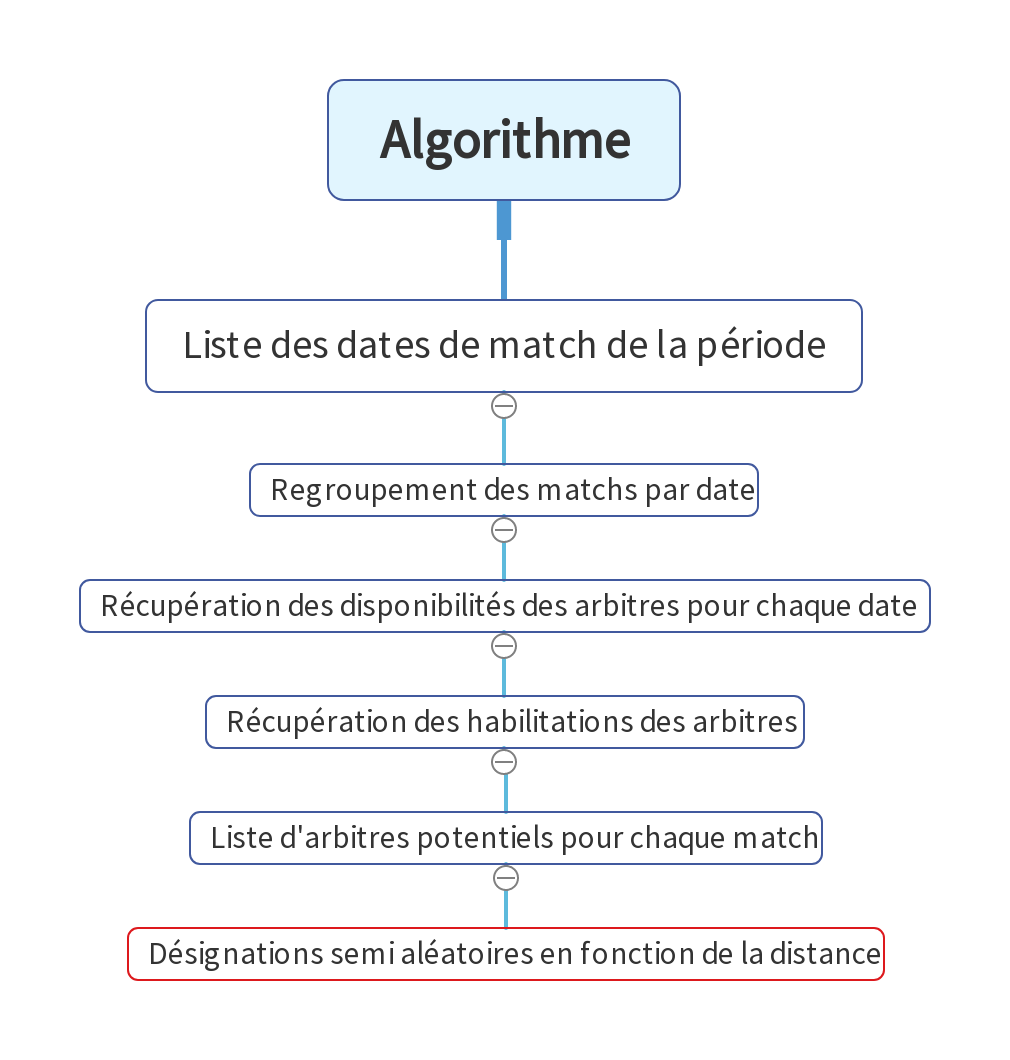
\includegraphics[height=15cm]{algorithme.png}
    \caption{Logique suivie par l'algorithme}
\end{figure}

